\documentclass[a4paper,11pt,titlepage,twoside,listof=totoc,bibliography=totoc,parskip=half]{scrbook}

% recommended defaults
\usepackage{babel}%
\usepackage[utf8]{inputenc}%
\usepackage[T1]{fontenc}
\usepackage{lmodern}
\usepackage{siunitx}
\usepackage{listings}
\usepackage{xcolor}
\usepackage[round]{natbib}   % omit 'round' option if you prefer square brackets
\bibliographystyle{plainnat}
\sisetup{per-mode=fraction}


% optional packages, yet recommended
\usepackage{amsmath,amssymb,amsthm} 
\usepackage{subcaption}
\usepackage{hyperref}
\usepackage{cleveref}
\usepackage{microtype}
\usepackage{booktabs}
\usepackage{graphicx}
\usepackage[style=english]{csquotes}
\usepackage{float}
\usepackage[section]{placeins}
\usepackage{derivative}
\usepackage{minted}
\usepackage{enumitem}
\usepackage{pgffor}
\usepackage{layouts}
\usepackage[colorinlistoftodos,prependcaption,textsize=tiny]{todonotes}

\usepackage[automark]{scrlayer-scrpage}
\pagestyle{scrheadings}

% configure some packages and macros
\usepackage{xspace}
\newcommand*{\zb}{z.B.\@\xspace}
\newcommand*\InputTable[1]{\input{./tables/#1.tex}}

\DeclareSIUnit\J{J}
\DeclareSIUnit\kb{k_B}
\newcommand*{\carry}[1][1]{\overset{#1}}
\newcolumntype{B}[1]{r*{#1}{@{\,}r}}
%\AddToHook{cmd/section/before}{\clearpage}
\graphicspath{ {../figures/} }

\title{Studying the Kosterlitz-Thouless Transition of the two-dimensional XY Model using Monte Carlo Methods}
\author{Lennart Voorgang}
\date{}
\publishers{\LARGE
	\begin{otherlanguage}{ngerman}
		Bachelorarbeit in Physik\\
		angefertigt am\\
		Helmholtz-Institut für Strahlen- und Kernphysik\\[3ex]
		vorgelegt der\\
		Mathematisch-Naturwissenschaftlichen Fakultät\\
		der\\
		Rheinischen Friedrich-Wilhelms-Universität\\
		Bonn\\[3ex]
		August 2025
	\end{otherlanguage}
	\vspace*{\fill}
}
\lowertitleback{%
	\begin{otherlanguage}{ngerman}
		I hereby declare that this thesis was formulated by me and that no sources or tools other than those cited were used.
		
		\vspace*{6ex minus 0.5ex}
		
		\begin{tabular}{@{}lc@{\hspace*{4.0cm}}c}
			Bonn, &  \makebox[3cm]{\dotfill} & \makebox[6cm]{\dotfill}\\
			& Date & Signature
		\end{tabular}
	\end{otherlanguage}
	
	\vspace*{10ex minus 4ex}
	
	\noindent
	\begin{otherlanguage}{ngerman}
		\begin{tabular}{@{}ll}
			1. Assessor: & Prof. Dr. Stefan Krieg \\
			2. Assessor: & Prof. Dr. Thomas Luu
		\end{tabular}
	\end{otherlanguage}
}


\newcommand{\Observable}[3]{\begin{figure}[htbp]
		\centering
		\includegraphics[width=0.8\textwidth]{../figures/#1/#2.pdf}
		\caption[Temperature dependence of the #3 per spin (#1)]{Temperature dependence of the #3 per spin using the #1 algorithm for lattice sizes $L \in \{4, 32, 128, 368\}$.}
		\label{fig:obs:#1:#2}
\end{figure}}

\newcommand{\Error}[3]{\begin{figure}[htbp]
		\centering
		\includegraphics[width=0.7\textwidth]{../figures/#1/#2_Errors.pdf}
		\caption[Temperature dependence of the #3 per spin errors (#1)]{Temperature dependence of the #3 per spin errors using the #1 algorithm for lattice sizes $L \in \{4, 32, 128, 368\}$.}
		\label{fig:obs:#1:#2:errors}
\end{figure}}

\newcommand{\Autocorrelation}[3]{\begin{figure}[htbp]
		\centering
		\includegraphics[width=0.8\textwidth]{../figures/#1/#2_Autocorrelation.pdf}
		\caption[Autocorrelation function $\Gamma(\Delta t)$ of the #3 per spin (#1)]{Autocorrelation function $\Gamma(\Delta t)$ of the #3 per spin using the #1 algorithm for $L=8$.}
		\label{fig:obs:#1:#2:autocorrelation}
\end{figure}}

\newcommand{\IntegratedAutocorrelation}[3]{\begin{figure}[htbp]
		\centering
		\includegraphics[width=0.8\textwidth]{../figures/#1/#2_IntegratedAutocorrelation.pdf}
		\caption[Integrated autocorrelation time $\tau$ of the #3 per spin (#1)]{Integrated autocorrelation time $\tau$ of the #3 per spin using the #1 algorithm for lattice sizes $L \in \{4, 32, 128, 368\}$.}
		\label{fig:obs:#1:#2:integrated}
\end{figure}}

\begin{document}
	\frontmatter
		\maketitle
		\tableofcontents
		\thispagestyle{empty}

	\mainmatter
		\pagenumbering{arabic}
		
		% Introduction
		\chapter{Introduction}\label{chap:introduction}
	In physics, there are a variety of problems for which it is either very hard or impossible to find analytical solutions. These problems often involve many particle systems and/or integrals of high dimensionality. With ever-increasing computing power available to researchers, it is becoming increasingly feasible to study such systems using Monte Carlo methods.
	
	The most well-known application of Monte Carlo methods in physics is the Ising model, a mathematical model commonly used to study phenomena such as phase transitions, critical temperatures, and universality. This model was first introduced and solved in one dimension by~\cite{ising} and later in two dimensions by~\cite{onsager}. It describes the total magnetization of a lattice as the superposition of all spin sites $\sigma_i = \pm 1$. It features a second-order phase transition at a critical temperature $T_C$, where the system transitions from an ordered low-temperature state to an unordered high-temperature state.
	
	One can now generalize the problem from a discrete $\mathbb{Z}_2$ symmetry to a continuous $U(2)$ symmetry. First introduced by~\cite{matsubara} as a model for liquid helium, it is now known as the XY model and it describes the spins as two-dimensional vectors on the unit circle. Unlike the Ising model, the XY model does not exhibit a second-order phase transition. However, as shown by~\cite{kosterlitz} (2016 Nobel Prize in Physics), it does feature something we now call a KT phase transition, where below a critical temperature $T_C$ metastable states can exist. These metastable states are closely related to vortex-antivortex pairs on the lattice, which annihilate as $T_C \rightarrow 0$.
	
	These kinds of systems are often simulated using the Metropolis-Hastings algorithm, which is prone to severe critical slowing-down effects. Cluster update algorithms introduced by~\cite{sw} and~\cite{wolff} reduce critical slowing-down effects and yield more accurate numerical results.
	
	In this bachelor's thesis, we employ Monte Carlo methods to study the two-dimensional XY model. The primary objective is to develop a program that simulates the XY model in a distributed manner, observes critical slowing-down effects when using the Metropolis-Hastings algorithm, and utilizes the Wolff cluster algorithm to mitigate them. The second goal is to observe the physical phenomena of the system, such as the KT phase transition, estimate the critical temperature $T_C$, and identify the annihilation of vortex-antivortex pairs.
	
		
		% Theoretical background
		\chapter{Theory}
		\section{XY Model}\label{sec:theo:xy_model}
	The XY model is the generalization of the Ising model where the spatial inversion symmetry $\sigma_i \rightarrow -\sigma_i$ ($\mathbb{Z}_2$) is replaced by a continuous $U(2)$ symmetry.
	
	\subsection{Definition}
		The XY model describes the spins $\sigma_i$ as two-dimensional vectors on the unit circle
		\begin{equation}\label{eq:hamiltonian}
			\sigma_i = \begin{pmatrix}
				\cos{\theta_i} \\ \sin{\theta_i}
			\end{pmatrix}
		\end{equation}
		parametrized by the angle $\theta_i \in [0,2\pi)$. The Hamiltonian gives the total energy of the system as
		\begin{equation}
			H = -J \sum_{\langle i, j \rangle}{s_i \cdot s_j} = -J \sum_{\langle i, j \rangle}{\cos(\Delta \theta)}
		\end{equation}
		where $\langle i,j \rangle$ are neighbouring spins, $\Delta \theta = \theta_i - \theta_j$ is the angle between two neighbouring spins, and $J>0$ is the interaction strength for the ferromagnetic case. The partition function for such a system is given by
		\begin{equation}
			Z = \sum{\exp{-\beta H}} = \sum{\exp{ \left( \beta J \sum_{\langle i, j \rangle}{\cos(\Delta \theta)} \right) }}
		\end{equation}
		with $\beta = (k_B T)^{-1}$ so that $[\beta] = \si{\per\joule}$ and $k_B$ being the Boltzmann constant. The coupling constant $J$ is set to $J = \SI{1}{\joule}$ so that $\beta J$ is dimensionless and $[H] = \si{\joule}$. 
		
	\subsection{Observables}
		For our studies, we use a square two-dimensional lattice with side length $L$, nearest neighbour approximation, and periodic boundary conditions, which, topologically, forms a torus. As the observables of the XY model scale with the number of lattice sites, it is generally more insightful to study the observables per spin. This way, the finite-size scaling of the observables can be observed more accurately.
	
		\paragraph{Energy per spin}
			The total energy of the system is given by its Hamiltonian and thus
			\begin{equation}\label{eq:energy}
				E = - \frac{1}{L^2} \sum_{\langle i, j \rangle}{\cos(\Delta \theta)}.
			\end{equation}
		
		\paragraph{Specific heat per spin}
			In addition to the energy per spin $E$, one can also record $E^2$ and derive the specific heat capacity of the system
			\begin{equation}\label{eq:specific_heat}
				C_V = \frac{\langle E^2 \rangle - \langle E \rangle^2}{T^2}.
			\end{equation}
		
		\paragraph{Magnetization per spin}
			The total absolute magnetization per spin for a system with side length $L$ is given by
			\begin{equation}\label{eq:magnetization}
				\lvert M \rvert^2 = \frac{1}{L^2} \left( (\sum{\cos\theta_i})^2 + (\sum{\sin\theta_i})^2 \right).
			\end{equation}
		
		\paragraph{Magnetic susceptibility}
			Similar to the specific heat, the magnetic susceptibility of the system can be derived as
			\begin{equation}\label{eq:magnetic_suceptibility}
				\chi = \frac{\langle M^2 \rangle - \langle M \rangle^2}{T}.
			\end{equation}
		
		\paragraph{Helicity modulus per spin}
			According to~\cite{teitel_helicity}, one can also derive the \emph{spin wave stiffness} or \emph{helicity modulus} $\Upsilon$, which \textquote{is a measure of the phase correlations of the system} (\cite[p. 598]{teitel_helicity}). It can be shown that the \emph{helicity modulus} is given by
			\begin{equation}\label{eq:helicity_modulus}
				\Upsilon = -\frac{1}{2} \langle E \rangle - \frac{J}{k_B T L^2} \left\langle \left(\sum_{\langle i,j \rangle}{\sin(\Delta \theta) \vec{r_{ij}} \cdot \vec{e}}\right)^2 \right\rangle
			\end{equation}
			\cite[eq. 3.2]{teitel_helicity} where, in addition to the existing definitions, $\vec{r}_{i,j}$ is the vector from site $i$ to site $j$ and $\vec{e}$ is an arbitrary unit vector. One may choose $\vec{e}$ such that it aligns along the rows of the lattice. Thus, only neighbours within a row contribute as $\vec{r}_{ij} \cdot \vec{e} = 0$ for neighbours outside the row.
	
	\subsection{Kosterlitz–Thouless Transition}
		Unlike the Ising model, the XY model does not feature a second-order phase transition of the usual kind, \enquote{as the ground state is unstable against low-energy spin-wave excitations} \cite[p. 1190]{kosterlitz}. It was shown by \cite{kosterlitz} that, instead, a transition now referred to as the KT phase transition occurs, where metastable states emerge below a critical temperature, $T_C$.
	
	\subsection{Vortices}
		These metastable states \enquote{correspond to vortices which are closely bound in pairs} \cite[p. 1190]{kosterlitz}. The vortex-antivortex pairs come closer together as the temperature decreases, until they pair-annihilate each other.
		\section{Numerical Methods}
	As stated in the introduction in~\cref{chap:introduction}, the goal is to simulate the two dimensional XY model with periodic boundary conditions using the Metropolis-Hastings and the Wolff-Cluster algorithms. In the following section I will present the concepts needed for understanding and implementing the simulation.
	
	\subsection{Importance Sampling}
		
		
	\subsection{Markov Chain}

	\subsection{Metropolis Algorithm}
	
	
		The overall procedure for the lattice is as follows:
		\begin{enumerate}
			\item Calculate $E$, $M$ and $\Upsilon$ for the initial lattice configuration.
			\item Perform a lattice sweep by iterating over all lattice sites. For every site $i$ do:
			\begin{enumerate}
				\item Propose a new angle $\theta_i \in [0,2\pi)$ from a uniform distribution.
				\item Calculate $\Delta H = \Delta E$, $\Delta M$ and $\Delta \Upsilon$ for the proposed new state.
				\item Accept or reject state with probability $P = \min{(1, \exp{(-\beta\Delta H)})}$.
			\end{enumerate}
			\item Update the observables $E \mathrel{{+}{=}} \Delta E$, $M \mathrel{{+}{=}} \Delta M$ and $\Upsilon \mathrel{{+}{=}} \Delta \Upsilon$ and add them to the result set.
			\item Repeat from 2. for a total of $N$ sweeps.
		\end{enumerate}
		
	\subsection{Critical Slowing Down}\label{sec:theo:critical_slowing_down}
		While the Metropolis-Hastings algorithms works well for low and high temperatures it has its problems near the critical temperature. 
		
	\subsection{Wolff Cluster Algorithm}\label{sec:theo:wolff_cluster}
		As discussed in~\cref{sec:theo:critical_slowing_down} the Metropolis-Hastings algorithm suffers severe critical slowing down effects. In a desire to mititage such effect~\cite{sw} introduced a multi-cluster Monte Carlo algorithm for the Potts spin models \enquote{giving a highly efficient method of simulation for large systems near criticality} (\cite{sw}).
		
		Adjacent to the multi-cluster Swendson and Wang algorithm, the Wollf algorithm shows similar improvements with regards to the critical exponent while only utilizing a single cluster which makes implementations more straight forward.
		
		The key insight is that the Ising spin-flip operation $\sigma_i \rightarrow -\sigma_i$ needs to be generalized to the $U(2)$ symmetry of the XY model. \cite{wolff} defines the spin-flip as the reflectionalong the hyperplane orthogonal to an arbritarly choosen unit vector $\vec{r}$
		\begin{equation}
			R(\vec{r}) \sigma_i = \sigma_i - 2 (\sigma_i \cdot \vec{r}) \vec{r} 
		\end{equation}
		which is an idempotent operation $R(\vec{r})^2=1$ \cite[eq. 3]{wolff}.
	
		The overall procedure for the Wolff cluster algorithm was taken from~\cite[p. 361]{wolff} with the addition of~\cref{wolf_loop}. This was done, as the probability of a site joining the lattice is lower for unordered states. These states emerge when the temperature is high and this the cluster size tends towards $1$. This results in a very uneven distribution of potential updates (\emph{marked} sites in the algorithm procedure). At low temperatures many sites get visited and potentionally updated while at high temperature as few as one site gets updated. To mitigate this, I introduce~\cref{wolf_loop} as an additional step which should ensure that even at high temperature a sufficient number of potential updates are made.
		\begin{enumerate}
			\item Calculate $E$, $M$ and $\Upsilon$ for the initial lattice configuration. Here the initial configuration is a cold state where $\sigma_i = 0$ for all sites $i$.
			\item \label{wolf_loop} Perform the following until we marked $L^2$ lattice sites in total:
			\begin{enumerate}
				\item Choose a random two dimensional unit vector $\vec{r}$ as the reflection vector.
				\item Pick a random lattice site $x$ as the first element of the cluster.
				\item Flip the spin at the initial lattice site $\sigma_x \rightarrow R(\vec{r}) \sigma_x$ and mark site $x$.
				\item \label{wolff_step} Visit all direct unmarked neighbours $y$ of $x$ and add them to the cluster with propbability
					\begin{equation}
						P(\sigma_x, \sigma_y) = 1 - \exp(\min[0, 2 \beta (\vec{r}\cdot\vec{\sigma_x}) (\vec{r}\cdot\vec{\sigma_y})])
					\end{equation}
					and calculate $\Delta E$, $\Delta M$ and $\Delta \Upsilon$ for the proposed new state.
				\item If site $y$ was accepeted into the cluster its spin is flipped $\sigma_y \rightarrow R(\vec{r}) \sigma_y$.
				\item Site $y$ becomes the new $x$ and continue from~\cref{wolff_step} until there are no more sites to add to the cluster.
			\end{enumerate}
			\item Update the observables $E \mathrel{{+}{=}} \Delta E$, $M \mathrel{{+}{=}} \Delta M$ and $\Upsilon \mathrel{{+}{=}} \Delta \Upsilon$ and add them to the result set.
			\item Continue from~\cref{wolf_loop} until the exit condition is fulfilled.
		\end{enumerate}
		
		
		
	
	\subsection{Bootstrapping}
		Since the Metropolis-Hastings algorithm scales with the number of lattice sites, it is computationally impractical to run the Metropolis-Hastings algorithm for long timescales. Given that we have an observable whose iid samples follow a Gaussian distribution and we already have \enquote{enough} iid samples which cover enough of the possible configuration space, we can then use bootstrapping to generate more samples (\citet{bootstrap}).
		\begin{enumerate}
			\item Collect $B$ intermediate means by repeating the following:
			\begin{enumerate}
				\item Take $A$ random samples from the blocked samples obtained in~\cref{sec:blocking} with replacement.
				\item Calculate the mean of those samples and add the result to the set of intermediate means.
			\end{enumerate}
			\item Calculate the final mean and the sample standard deviation of those $B$ intermediate means.
		\end{enumerate}
		
		% Implementation
		\chapter{Implementation}
\section{General}
			\section{Procedure}
	We propose and implement the following procedure to mitigate aforementioned shortcomings. The various subsystems of the simulation are described in \Cref{sec:impl:scanning,sec:impl:computing,sec:impl:tasks}.
	
	The high-level procedure is as follows:
	\begin{enumerate}
		\item The database schema (\Cref{chap:schema}) is initialized by the compute nodes in~\Cref{sec:impl:computing:compute}.
		\item The compute nodes read the configuration file from the current working directory.
		\item \label{procedure_loop} The temperature interval is divided into steps according to~\cref{scanning:init} of~\Cref{sec:impl:scanning}. The resulting configurations are inserted into the database if they do not already exist.
		\item \label{procedure_pipeline} The program checks whether any existing configuration is incomplete and, if so, executes the task pipeline defined in~\Cref{sec:impl:tasks}.
		\item One of the compute nodes simulates the annihilation of the vortex/antivortex pair.
	\end{enumerate}
	Note that~\cref{procedure_loop,procedure_pipeline} can repeat multiple times. This is defined by the scanning depth which will be discussed in the following section.


				\section{Temperature Scanning}
				\subsection{Distributed Computing}\label{sec:impl:computing}
	The temperature scanning of~\Cref{sec:impl:scanning} divides every lattice size $L$ into $N$ steps and $I$ iterations. As the number of configurations far exceeds the core count of a single computer for any realistic choice of $L$, $N$, and $I$, the computational efforts should be scaled out across multiple compute nodes. The implementation addresses the shortcomings mentioned at the beginning of~\Cref{sec:impl} and requires two kinds of nodes.
	
	\subsubsection{Data Node}\label{sec:impl:computing:data}
		The \emph{data} node is responsible for orchestrating the compute nodes and storing the intermediate and final results. The orchestration is realized using a  \emph{PostgreSQL}\footnote{\url{https://www.postgresql.org}} database and does not require any additional software. Having a central \emph{data} node fixes shortcoming~\cref{shortcomings:sqlite}, where the nodes need to have access to a common network share.
		
		The schema for the \emph{PostgreSQL} database is presented in~\Cref{chap:schema}. Foreign keys link all relevant database entities, and unique constraints have been added to ensure that every configuration is simulated exactly once.
	
	\subsubsection{Compute Node}\label{sec:impl:computing:compute}
		One or more \emph{compute} nodes are required to run the simulation. These nodes should have modern, high-frequency, multi-core CPUs with \emph{AVX2} support (\cref{sec:impl:optimizations}) as our simulation primarily utilizes the CPU.
		
		The compute nodes only need internal network access to the \emph{data} node to access the \emph{PostgreSQL} instance. To automatically install all required dependencies and compile the program, a \emph{CloudInit}\footnote{\url{https://cloudinit.readthedocs.io/en/latest/index.html}} configuration file is available in the repository\footnote{\url{https://github.com/lennartvrg/physik690-Bachelorarbeit/blob/main/cloud-config.yaml}}. The script also registers the program as a \emph{systemd}\footnote{\url{https://systemd.io/}} service, which provides resilience by restarting the service when it exits with an error code\footnote{\url{https://github.com/lennartvrg/physik690-Bachelorarbeit/blob/main/bachelor.service}}.

				\subsection{Task-based Scheduler}\label{sec:impl:tasks}
	As each \emph{compute} node has multiple cores, the workload can be distributed across them. These so-called worker threads work on the following tasks until there are no more tasks available.
	\begin{enumerate}
		\item In the \emph{simulation} task, the worker thread simulates a configuration, thermalizes and blocks the results, and writes back the iid samples of $E$, $E^2$, $M$, $M^2$, and $\Upsilon$ to the database. Additionally the final spin arrays are also written to the database, which fixes shortcomings~\cref{shortcomings:bootstrap,shortcomings:sweeps}.
		\item In the \emph{bootstrap} task, the worker threads retrieve the iid samples for each configuration that was simulated beforehand. The samples are bootstrapped, and the final results are written to the database.
		\item In the \emph{derivative} task, the workers calculate the observables ($C_V$, $\chi$) derived from the bootstrapped results.
	\end{enumerate}
	These steps are executed in stages, so initially, all worker threads focus on \emph{simulation} tasks until none remain. As soon as all the compute nodes' worker threads have finished with one type of task, they can proceed to the following kind of task. Note that the worker threads may work on configurations belonging to different lattice sizes, which fixes shortcoming~\cref{shortcomings:cores}.
	
	As the pipeline finishes, the \emph{compute} nodes wait for each other in a synchronization step. From here, they go back to~\cref{scanning:iter} of the temperature scanning procedure. If the exit condition $I_C \ge I_\text{max}$ is fulfilled, the \emph{compute} nodes exit.

	\subsubsection{Chunking}\label{sec:impl:tasks:chunks}
		The \emph{simulation} task uses chunking to alleviate~\cref{shortcomings:crashed} discussed earlier in the chapter. The total number of sweeps is defined here as the product of the number of sweeps per chunk and the number of chunks $N_\text{Chunks}$, which can be set in the config file. The worker threads work on a given configuration, one chunk at a time, and write back the intermediate results and the current spins to the database. This way, another worker can continue working on a configuration when the original worker crashes. Splitting the workload into chunks ensures that if a node should fail, only a subset of iid samples is lost.

	\subsubsection{Scheduling}
		A task scheduler was implemented, which delegates the workload to the worker threads. The number of worker threads equals the number of CPU cores available to the program. A dedicated scheduling thread is started, which connects to the database. The task distribution works as follows:
		\begin{enumerate}
			\item The worker threads register themselves as available.
			\item \label{scheduler_loop} The scheduling thread searches for any available worker threads.
				\begin{enumerate}
					\item If a worker is available, the next task is fetched and delegated to the available worker.
					\item If no worker is available, the scheduling thread sleeps for one second.
				\end{enumerate}
			\item The scheduling tasks check if the worker threads have published any results and write them to the database.
			\item Go to~\cref{scheduler_loop} unless all workers are waiting and no new tasks are available.
		\end{enumerate}
			\section{Optimizations}\label{sec:impl:optimizations}
	Apart from distributing the workload across multiple threads and nodes, some optimizations can be made to improve performance on a single thread.
	
	\paragraph{SIMD Instructions}\label{sec:impl:optimizations:simd}
		As already introduced in the definitions of the Metropolis (\cref{sec:theo:metropolis}) and Wolff (\cref{sec:theo:wolff_cluster}) algorithms, it is computationally more sensible to calculate the delta energy/magnetization/helicity modulus that a proposed spin update would entail, instead of recalculating the observable for the entire lattice. In our two-dimensional lattice model with nearest neighbour approximation, this means that only the four direct neighbours of a spin $\sigma_i$ contribute to the calculation.
			
		As many modern-day CPUs have the AVX2\footnote{\url{https://edc.intel.com/content/www/us/en/design/ipla/software-development-platforms/client/platforms/alder-lake-desktop/12th-generation-intel-core-processors-datasheet\\-volume-1-of-2/009/intel-advanced-vector-extensions-2-intel-avx2/}} instruction set enabled, which allows us to perform standard mathematical operations on vectors of four $64$-bit scalars simultaneously, we can use this to improve the performance of our implementation. \emph{AVX2} in itself does not provide intrinsics for the operations ($\sin, \cos$) that are needed. Therefore, we will also use the \emph{Intel\textsuperscript{\tiny\textregistered} Short Vector Math Library} (SVML\footnote{\url{https://www.intel.com/content/www/us/en/docs/cpp-compiler/developer-guide-reference/2021-8/intrinsics-for-short-vector-math-library-ops.html}}), which provides methods that generate an optimized sequence of intrinsics for $\sin$ and $\cos$.
		
		To optimize data access for our SIMD instructions, the internal \mintinline{c++}{std::vector<double_t>} storing the spins is aligned on a $32$-byte boundary.
		
	\paragraph{Compiler Flags}
		The program uses the \mintinline{bash}{-march=native} compiler flag and should therefore be compiled on a system with the same or very similar CPU as the compute nodes. Additionally, the \mintinline{bash}{-ffast-math} flag was used, which sacrifices ISO compliance for execution speed. Although no systematic testing was conducted, the performance improvement on the development machine was $\approx \SI{20}{\percent}$ better, with no observable loss in numerical results. 
	
	\paragraph{Intel Compiler}
		We also wanted to try the \emph{Intel\textsuperscript{\tiny\textregistered}} oneAPI DPC++/C++ compiler as the manufacturer claims it offers superiority over \emph{gcc} in HPC workloads. No systematic testing was conducted, but on the development machine (AMD Ryzen 1700) a $\SI{6}{\percent}$ reduction of the total wall-time was observed. Tests on a second machine (\emph{Intel\textsuperscript{\tiny\textregistered} i7-10710U}) yielded a $\SI{14}{\percent}$ improvement over $\emph{gcc 15}$.
			
	


	
			
			% Results
			\chapter{Results}
	The following results were obtained from a run on a cluster with eight nodes, each with $16$ cores. The simulation was configured to run for lattice sizes $L \in \{4, 8, 16, \dots, 378\}$\footnote{Full list: $\{4, 8, 16, 32, 48, 64, 80, 96, 112, 128, 144, 160, 176, 192, 208, 224, 240, 256, 272, 288, 304, 320,\\336, 352, 378\}$}. The initial setup is a cold state where $\sigma_i = 0$ for all sites $i$, $\num{200000}$ bootstrap resamples and a scanning depth of two. Each chunk performed $\num{50000}$ sweeps, with the number of chunks depending on the algorithm.
	\begin{enumerate}
		\item For the Metropolis algorithm, $\num{32}$ chunks were used, resulting in a total of $\num{1600000}$ sweeps.
		\item For the Wolff algorithm, six chunks were used, resulting in a total of $\num{300000}$ sweeps.
	\end{enumerate}
	These numbers were chosen as initial, smaller-scale runs during development suggested that the Wolff algorithm suffers significantly less from the critical slowing down effect, resulting in more accurate results even with fewer sweeps. The simulation ran for five days on the aforementioned cluster.
	
	The following sections will discuss the results and derive estimates for the critical temperature $T_C$. Note that for the discussion of the observables, the focus will be on a subset of lattice sizes $L \in \{4, 32, 128, 352\}$ so as not to clutter the plots more than necessary. The plots for all observables at all lattice sizes may be found in the repository (see~\cref{chap:source_code}).
	
	\section{Cluster Size}\label{sec:res:cluster_size}
		Some of the observations we will make in the following sections will only be explainable with the average cluster size. This observable is exclusive to the Wolff algorithm and is plotted in~\Cref{fig:obs:Wolff:ClusterSize}. The observable is dependent on the lattice size, as the maximum number of sites a cluster may have is at maximum equal to the total number of lattice sites.
		
		Taking into account the acceptance probability $P(\sigma_x, \sigma_y)$ (\cref{eq:wolff}) of the Wolff algorithm, it also makes sense that at low temperatures almost the entire lattice is part of the cluster. As the temperature increases, the average cluster size experiences a sharp dropoff, which is more pronounced for larger lattice sizes. For high temperatures, the average cluster size tends towards $\num{1}$ for all latices sizes. An essential aspect is that the dropoff happens after the point where we expect the critical temperature $T_C$ to be. If this were not the case, the Wolff algorithm would not yield an improvement over the Metropolis algorithm when estimating $T_C$.
		
		The observation that the average cluster tends towards $\num{0}$ when $T\rightarrow \infty$ also justifies the introduction of~\cref{wolf_loop} in~\cref{sec:theo:wolff_cluster}. If we did not do that, the lattice would not be given enough chances to update, which, at high temperatures, would result in a highly correlated observable. Correlated observables, in turn, would result in a larger integrated autocorrelation time $\tau$. As we use $\lceil \tau \rceil$ to block the intermediate results, it would also reduce the accuracy and precision of our final estimates, since we have fewer iid samples.
		\Observable{Wolff}{ClusterSize}{average cluster size}
	
			\section{Energy}\label{sec:res:energy}
	\subsection{Observable}\label{sec:res:energy:observable}
		\Observable{Metropolis}{Energy}{energy}
		\Observable{Wolff}{Energy}{energy}
		\Cref{fig:obs:Metropolis:Energy} shows the temperature dependence of the energy per spin (\cref{eq:energy}) using the Metropolis algorithm. We observe the expected quasi-ordered state at low temperatures, where the spins mostly align. The energy tends towards $\SI{-2}{\joule}$ for $T\rightarrow 0$, which matches the Ising model. With increasing temperature, the absolute value of the energy per spin slowly reduces. For $T \rightarrow \infty$ we can expect $E \rightarrow 0$ as the spins become less and less aligned, and the spin energies average out. The errors can be found in~\Cref{sec:errors:energy} of~\Cref{chap:errors}.
		
		Comparing the form of the curve with the results of the Wolff algorithm in~\Cref{fig:obs:Wolff:Energy} shows the same overall form. A slight deviation can be observed for $L = 4$, where at $T = \SI{3}{\joule\per\kb}$, the data point for the Wolff algorithm is slightly lower than that for the Metropolis algorithm. The lower data point is probably due to the small lattice size and the fact that cluster sizes tend towards one at higher temperatures (see~\cref{sec:res:cluster_size}). At these higher temperatures, the acceptance probabilities of both algorithms are smaller, and, as the Wolff algorithm always flips at least one site (the starting site of the cluster-building procedure), we obtain a slightly different curve compared to the Metropolis algorithm, as the Metropolis algorithm may flip as few as zero spins.
		
		While the energy per spin curve is visually the same for both algorithms, the residuals and integrated autocorrelation time $\tau$ differ significantly. We plotted the autocorrelation function $\Gamma(\Delta t)$ at the lowest, highest, and the temperature where  the magnetic susceptibility $\chi$ peaked. The autocorrelation function was cut off at the last datapoint where $\Gamma(\Delta t) > \num{0}$.
		
		Comparing the Metropolis algorithm (\cref{fig:obs:Metropolis:Energy:autocorrelation}) and the Wolff algorithm (\cref{fig:obs:Wolff:Energy:autocorrelation}) reveals that low temperatures generally exhibit autocorrelation function curves with long tails. In contrast, high temperatures feature a short autocorrelation curve. Near criticality, the autocorrelation function approaches zero much more quickly when using the Wolff algorithm. This behaviour is expected as the Wolff algorithm is supposed to give \enquote{a highly efficient method of simulation for large systems near criticality}~\cite[p. 86]{sw}.
		\Autocorrelation{Metropolis}{Energy}{energy}
		\Autocorrelation{Wolff}{Energy}{energy}
		
		The advantage becomes even clearer when plotting the integrated autocorrelation time $\tau$ of the Metropolis algorithm (\cref{fig:obs:Metropolis:Energy:integrated}) and the Wolff algorithm (\cref{fig:obs:Wolff:Energy:integrated}). When comparing these graphs, we can see that $\tau$ is much smaller when using the Wolff algorithm. As already discussed in~\Cref{sec:res:cluster_size}, this results in more iid samples and a more accurate and precise measurement of our observables. We conclude that the Wolff algorithm suffers less from critical slowing and yields superior estimates of our observables in terms of accuracy and precision.
		\IntegratedAutocorrelation{Metropolis}{Energy}{energy}
		\IntegratedAutocorrelation{Wolff}{Energy}{energy}
	
	\paragraph{Energy squared per Spin}\label{sec:res:energysquare} A thorough discussion of $E^2$ will be omitted as the general observations of $E$ also hold for $E^2$. The plots are, for completeness' sake, enclosed in~\Cref{sec:observables:energy_squared}, and the errors can be found in~\Cref{sec:errors:energysquare} of~\Cref{chap:errors}..
	
	\subsection{Specific Heat}\label{sec:res:cv:observable}
		The specific heat capacity $C_V$ can be derived from $\langle E \rangle$ and $\langle E^2 \rangle$  using~\Cref{eq:specific_heat}. Comparing $C_V$ using the Metropolis (\cref{fig:obs:Metropolis:SpecificHeat}) and Wolff (\cref{fig:obs:Wolff:SpecificHeat}) algorithms reveals that both follow the same curve. The specific heat per spin starts small, has a small peak which moves closer to $T_C$ with increasing lattice sizes, and then falls off for $T\rightarrow 0$. The errors can be found in~\Cref{sec:errors:specificheat} of~\Cref{chap:errors}.
		
		Near criticality, the curve of $C_V$ obtained using the Wolff algorithm is substantially smoother, which can be attributed to the reduced critical slowing-down effects experienced by the Wolff algorithm.
		\Observable{Metropolis}{SpecificHeat}{specific heat}
		\Observable{Wolff}{SpecificHeat}{specific heat}
	
	\subsection{Helicity Modulus}\label{sec:res:helicity:observable}
		As introduced in~\Cref{eq:helicity_modulus}, the helicity modulus $\Upsilon$ \enquote{measures the increase in the amount of energy when we rotate the order parameter of a magnetically long-range-order system along a given direction by a small angle} \citep[p. 1]{krueger}. Comparing the curves of Metropolis (\Cref{fig:obs:Metropolis:HelicityModulus}) and Wolff (\Cref{fig:obs:Wolff:HelicityModulus}) reveals no difference in overall form, although the curve obtained using the Wolff algorithm is smoother. For $T \rightarrow 0$, the XY model has a long-range order, and the helicity modulus $\Upsilon$ tends towards $1$. Above $T_C$, the long-range order vanishes and $\Upsilon$ drops towards $0$. The errors can be found in~\Cref{sec:errors:helicity} of~\Cref{chap:errors}.
		\Observable{Metropolis}{HelicityModulus}{helicity modulus}
		\Observable{Wolff}{HelicityModulus}{helicity modulus}
		
		One particular feature of the helicity modulus is that the intersection of the graph of $\frac{2}{\pi} T$ and $\Upsilon$ can be used to estimate $T_C$~\citep{teitel_helicity}. Attempts by~\cite{teitel_helicity} and~\cite{olsson_helicity} show that while this is possible, the results are generally less precise than using the magnetic susceptibility $\chi$ to estimate $T_C$. We will therefore concentrate on the latter in the following sections.

	
			\section{Magnetization}\label{sec:res:magnet}
	\subsection{Observable}\label{sec:res:magnet:observable}
		\Observable{Metropolis}{Magnetization}{magnetization}
		\Observable{Wolff}{Magnetization}{magnetization}
		Studying the total absolute magnetization per spin for the Metropolis (\cref{fig:obs:Metropolis:Magnetization}) and Wolff (\cref{fig:obs:Wolff:Magnetization}) algorithms shows that, for low temperatures, the magnetization tends to $1$, indicating the existence of a quasi-ordered low-temperature state. With increasing temperature, the magnetization decreases steadily at first and then rapidly until it slowly levels out in the unordered high-temperature state. One can also see finite-size effects as, for increasing lattice sizes, the form of the curve becomes more pronounced. The errors can be found in~\Cref{sec:errors:magnetization} of~\Cref{chap:errors}.
		
		\paragraph{Magnetization Squared per Spin}\label{sec:res:magnetsquare} The plots for the absolute total magnetization per spin, its autocorrelation function, and integrated autocorrelation time can be found in~\Cref{sec:observables:magnetization_squared}, and the errors can be found in~\Cref{sec:errors:magnetizationsquare} of~\Cref{chap:errors}.
	
	\subsection{Magnetic Susceptibility}\label{sec:res:xs}
		\Observable{Metropolis}{MagneticSusceptibility}{magnetic susceptibility}
		\Observable{Wolff}{MagneticSusceptibility}{magnetic susceptibility}
		The magnetic susceptibility $\chi$ can be derived from $\langle M \rangle$ and $\langle M^2 \rangle$ according to~\Cref{eq:magnetic_suceptibility}.  Comparing the curve of the Metropolis (\cref{fig:obs:Metropolis:MagneticSusceptibility}) and Wolff (\cref{fig:obs:Wolff:MagneticSusceptibility}) algorithms reveals a similar form. The magnetic susceptibility is small for low and high temperatures. A peak exists near the critical temperature, which slowly shifts to the left and becomes narrower as the lattice size increases and the peak's magnitude decreases. The errors can be found in~\Cref{sec:errors:magneticsusceptibility} of~\Cref{chap:errors}.
		
		Near criticality, the curve of $X$ obtained using the Wolff algorithm is substantially smoother, which can be attributed to the reduced critical slowing down effects experienced by the Wolff algorithm.
	
	\subsection{Estimating \texorpdfstring{$T_C$}{T} using the Magnetic Susceptibility \texorpdfstring{$\chi$}{X}}\label{sec:res:temperature}
		As shown by~\citet[eq. 3]{shifted}, there exists a shifted temperature $T^*$ that asymptotically approaches the critical temperature $T_C$ for an infinite lattice
		\begin{equation}\label{eq:shifted_temperature}
			T^*(L) \approx T_C + \frac{\pi^2}{4c (\ln{L})^2}.
		\end{equation}
		The shifted temperature gives us a way to estimate the critical temperature $T_C$. To confirm the correlation between lattice size and shifted temperature, we now take the maximum magnetic susceptibility $\chi_\text{max}$ per lattice size from~\Cref{fig:obs:Metropolis:MagneticSusceptibility} and plot the temperature $T$ where it occurs against $(\ln{L})^{-2}$ in~\Cref{fig:critical_temperature}.
		\begin{figure}[htbp]
			\centering
			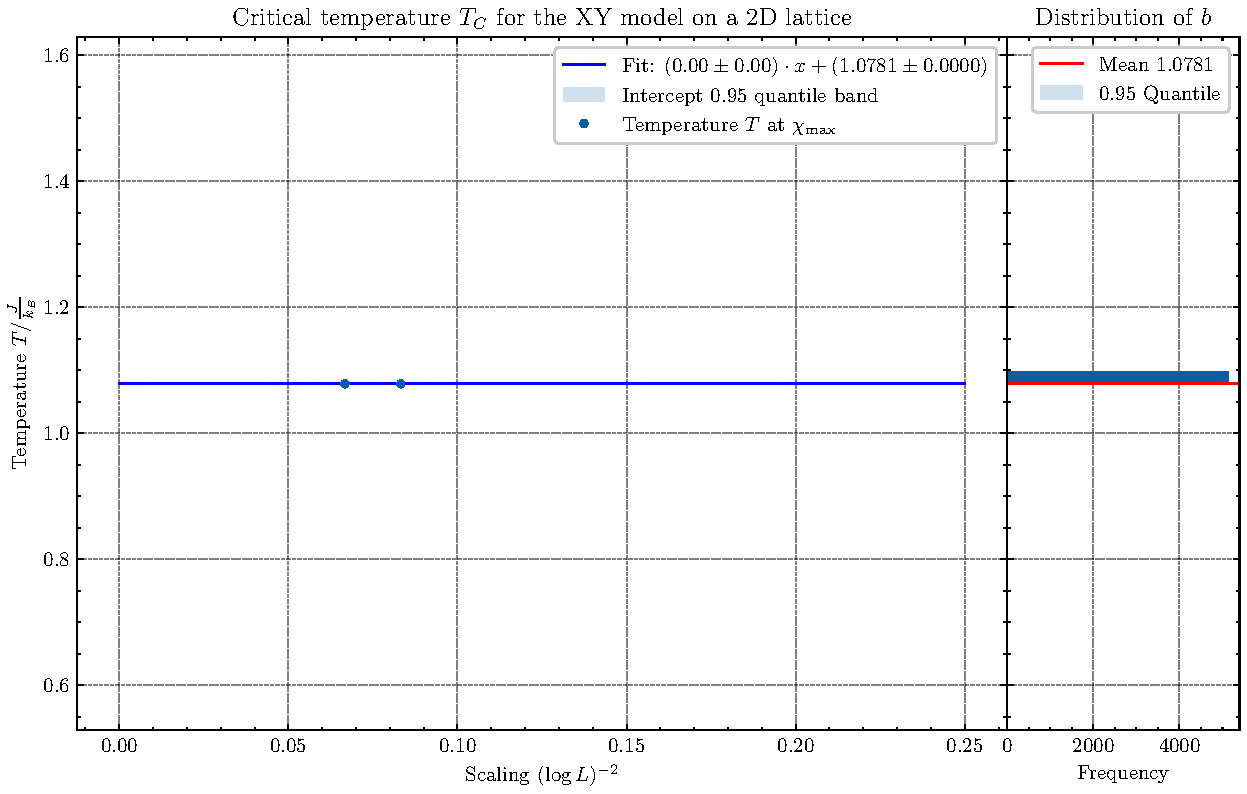
\includegraphics[width=0.8\textwidth]{../figures/Metropolis/Critical_Temperature.pdf}
			\caption[Estimating $T_C$ using the Metropolis algorithm by plotting $T$ where $\chi$ is maximal against $(\ln L)^{-2}$]{The temperature at which $\chi$ is maximal against $(\ln L)^{-2}$ yields a linear correlation and confirms~\Cref{eq:shifted_temperature} for the Metropolis algorithm.}
			\label{fig:critical_temperature}
		\end{figure}
		\begin{figure}[htbp]
			\centering
			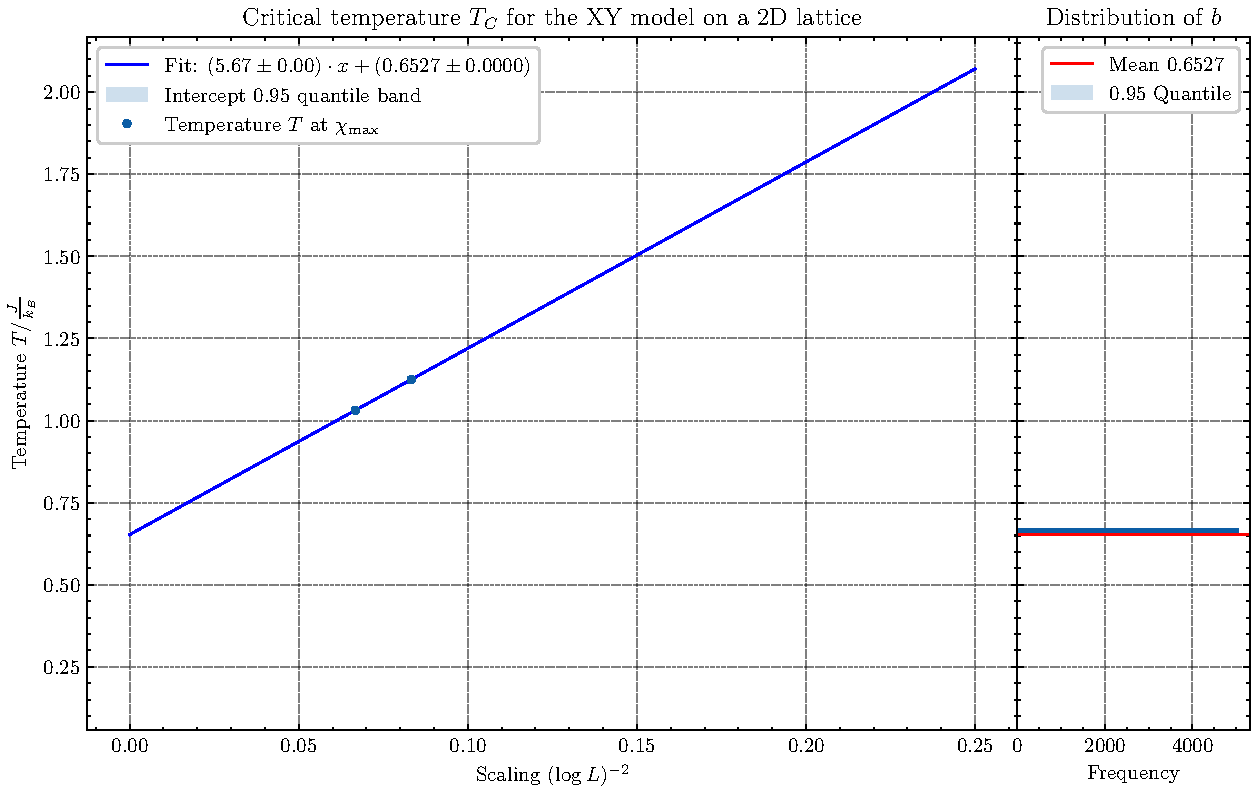
\includegraphics[width=0.8\textwidth]{../figures/Wolff/Critical_Temperature.pdf}
						\caption[Estimating $T_C$ using the Wolff algorithm by plotting $T$ where $\chi$ is maximal against $(\ln L)^{-2}$]{The temperature at which $\chi$ is maximal against $(\ln L)^{-2}$ yields a linear correlation and confirms~\Cref{eq:shifted_temperature} for the Wolff algorithm.}
			\label{fig:critical_temperature_wolf}
		\end{figure}
		
		We fitted a linear regression model using a least-squares method against our data points, which confirms the correlation of lattice size and shifted temperature. The intercept of the fit gives the estimate for the critical temperature. To estimate our errors, we used a bootstrap approach by resampling $\num{10 000}$ times from our measurements and redoing our linear regression model each time. As seen on the right side of~\Cref{fig:critical_temperature}, the distribution of intercepts $b$ follows a Gaussian distribution and therefore the central limit theorem. The standard deviation $\sigma$ of our bootstrapped intercepts was taken as the error of our estimate of the critical temperature
		\begin{equation}
			T_{C, \text{Metropolis}} = \SI{0.886(12)}{\J\per\kb}.
		\end{equation}
		Doing the same for the Wolff algorithm (\cref{fig:critical_temperature_wolf}) for our $\chi_\text{max}$ obtained from~\Cref{fig:obs:Wolff:MagneticSusceptibility} yields
		\begin{equation}
			T_{C, \text{Wolff}} = \SI{0.8978(14)}{\J\per\kb}.
		\end{equation}
		Comparing the two estimates shows that the Wolff algorithm yielded a more precise measurement. The increase in precision can be attributed to the reduced critical slowing-down effects experienced by the Wolff algorithm.
		
		We can compare our result with some literature values:
		\begin{itemize}
			\item In~\citet{literature_gpu}, the authors used a GPU-based Monte Carlo approach to estimate the critical temperature to $T_C=\SI{0.8935(1)}{\J\per\kb}$.
			\item In~\citet{literature_cpu}, the authors used a CPU-based Monte Carlo approach to estimate the critical temperature to $T_C=\SI{0.89213(10)}{\J\per\kb}$.
			\item A theoretical transfer matrix approach employed by~\cite{literature_theo} led to a critical temperature of $T_C \approx \SI{0.8916}{\J\per\kb}$.
		\end{itemize}
		These literature values are compatible with our estimated $T_{C, \text{Metropolis}}$ which indicates that our implementation is correct and our temperature \emph{zoom} procedure works. Our errors are bigger by a factor of $\sim 100$ than those of others, which is a result of our time and resource constraints. The errors of our estimate $T_{C, \text{Wolff}}$ are smaller by a factor of $\sim 10$ than those of the Metropolis algorithm, which is another indication of the superiority of the Wolff algorithm near the critical temperature. The estimate itself is numerically larger than expected, and the literature values are therefore outside of our errors. This is not surprising, as the literature values were, at least for those obtained using Monte Carlo methods, simulated on larger lattice sizes ($L = 512$) and used more mathematical insights when fitting $\chi$.

		When zooming in on the $\chi$ peak for the Metropolis (\cref{fig:critical_temperature_zoom}) and Wolff (\cref{fig:critical_temperature_wolf_zoom}) algorithms, we see further advantages of  using the Wolff algorithm. The data points follow a very predictable trajectory,  which gives us the confidence that if we were to increase the temperature scanning depth to $\geq 3$, we would not zoom in on the wrong neighbourhood.
		\begin{figure}[htbp]
			\centering
			\includegraphics[width=0.8\textwidth]{../figures/Metropolis/Critical_Temperature_Zoom.pdf}
			\caption[Estimating $T_C$ using the Metropolis algorithm by plotting $T$ where $\chi$ is maximal against $(\ln L)^{-2}$]{The temperature at which $\chi$ is maximal against $(\ln L)^{-2}$ yields a linear correlation and confirms~\Cref{eq:shifted_temperature} for the Metropolis algorithm.}
			\label{fig:critical_temperature_zoom}
		\end{figure}
		\begin{figure}[htbp]
			\centering
			\includegraphics[width=0.8\textwidth]{../figures/Wolff/Critical_Temperature_Zoom.pdf}
			\caption[Estimating $T_C$ using the Wolff algorithm by plotting $T$ where $\chi$ is maximal against $(\ln L)^{-2}$]{The temperature at which $\chi$ is maximal against $(\ln L)^{-2}$ yields a linear correlation and confirms~\Cref{eq:shifted_temperature} for the Wolff algorithm.}
			\label{fig:critical_temperature_wolf_zoom}
		\end{figure}

			\section{Vortex Unbinding}\label{sec:vortex_unbinding}
	To visualize the vortex unbinding at low temperatures, we performed a single run where we first heated a $64 \times 64$ lattice  to $T = \num{1.5}$ and allowed it to thermalize for $\num{100 000}$ sweeps. The temperature was then lowered back down to $T = \num{0.05}$ in $90$ steps with $20$ sweeps of thermalization at each temperature step. At $T = \num{0.05}$, the system was given $\num{90 000}$ sweeps to allow the vortices to unbind. An animation of the procedure can be viewed here\todo{Upload to some video platform}, with some key frames shown  \todo{Still need to export them from the animation and put them in the appendix}
	
	Below the critical temperature $T_C$, bound vortex-antivortex pairs appear. As the temperature is further lowered, the pairs come closer together until they annihilate. The lattice is left in a quasi-ordered low-temperature state.
			\section{Scaling}\label{sec:scaling}
	\begin{figure}[htbp]
		\centering
		\includegraphics[width=0.8\textwidth]{../figures/Scaling.pdf}
		\caption[Correlation of the computational effort and the lattice size]{Lattice size dependence of the total computation time of the Metropolis and Wolff algorithms}
		\label{fig:scaling}
	\end{figure}
	In~\Cref{fig:schema}, we observe that the total simulation time $T$ is proportional to $L^2$. The Wolff algorithm takes $\sim \frac{1}{2}$ the time of the Metropolis while, as discussed in~\Cref{sec:res:temperature}, coming to a more precise estimate. As the Metropolis algorithm used $24$ chunks and the Wolff algorithm only $6$ chunks, we conclude that the cluster building procedure of the Wolff algorithm is computationally more expensive than a single sweep of the Metropolis procedure. Note that the simulation ran on a compute cluster in the public cloud, so we cannot account for the effects of noisy neighbours and other external factors.
			
			% Conclusion
			\chapter{Conclusion}
	In this work, we implemented a program that simulates the XY model using the Metropolis (\cref{sec:theo:metropolis}) and Wolff (\cref{sec:theo:wolff_cluster}) algorithms. The simulation was able to combine the computational resources of an eight-node cluster effectively, which is a promising indicator for future runs on bigger clusters.
	
	We were able to study the per spin observables energy $E$ (\cref{sec:res:energy:observable}), specific heat $C_V$ (\cref{sec:res:cv:observable}), total absolute magnetization $\lvert M^2 \rvert$ (\cref{sec:res:magnet:observable}), and magnetic susceptibility $\chi$ (\cref{sec:res:xs}). Additionally, we observed critical slowing-down effects in~\Cref{sec:res:energy:observable} and, by implementing the Wolff single cluster algorithm, successfully reduced them.
	
	In~\Cref{sec:res:temperature}, we used the shifted temperature $T^*$~\citep{shifted} to estimate the critical temperature $T_C$ for the Metropolis algorithm to:
	\begin{equation}
			T_{C, \text{Metropolis}} = \SI{0.8902(118)}{\J\per\kb}.
	\end{equation}
	For the Wolff algorithm, we were also able to account for the choice of $L$ and got the estimate:
	\begin{equation}
			T_{C, \text{Wolff}} = \SI{0.8934(9)}{\J\per\kb}.
	\end{equation}
	The errors were obtained from a bootstrap procedure using the standard deviation $\sigma$. As discussed in~\Cref{sec:res:temperature}, both of our estimates are compatible with existing literature values, although the Metropolis estimate might only be compatible on account of the large errors. The Wolff algorithm is in particular good agreement with the literature values. The errors obtained using the Wolff algorithm were smaller by a factor of $\approx 10$ than those of the Metropolis algorithm, which indicates the reduced effects of critical slowing-down.
	
	In~\Cref{sec:vortex_unbinding}, we observed the existence and annihilation of vortex-antivortex pairs below the critical temperature $T_C$ when using the Metropolis algorithm. For the Wolff algorithm, the vortex-antivortex pairs dissolve too quickly to visualize.
	
	At last, in~\Cref{sec:scaling}, we discussed the correlation of computational effort and lattice size, and we found the total simulation time $T$ to be proportional to $L^2$.
	
	\section{Outlook}
		If we were to continue this project with the intent of finding a better estimate of the critical temperature, we would rely solely on the Wolff algorithm, as it gives more accurate estimates in a shorter amount of time. As the $\chi$ peaks get smaller with increasing lattice sizes, we would increase the temperature scanning depth from $2$ to $3$ or $4$. Combined with more simulated chunks and increased $L$, this should result in better estimates.
		
		The further use of the Metropolis algorithm using a CPU approach does not promise better results, as we would need to increase the number of chunks too much to still obtain usable $\chi$ peaks. However, many papers \citep*{literature_gpu} were quite successful in parallelizing the Metropolis on the GPU. A comparison of Wolff on the CPU and Metropolis on the GPU would be an interesting topic of further research.
		
			
		\cleardoubleemptypage
		
	\appendix
		\chapter{Source Code}\label{chap:source_code}
	The program requires the installation of a \emph{gcc}\footnote{\url{https://gcc.gnu.org/}} or \emph{Intel\textsuperscript{\tiny\textregistered} oneAPI DPC++/C++ Compiler}\footnote{\url{https://www.intel.com/content/www/us/en/developer/tools/oneapi/dpc-compiler.html}}, with support for \emph{C++26}. The build process was tested with versions 15.1.1 and 2025.0.4, respectively. The source code for the simulation, as well as the sources for this report, can be obtained from GitHub:
	\begin{center}
		\url{https://github.com/lennartvrg/physik690-Bachelorarbeit}
	\end{center}
	As the program makes use of submodules, it is necessary to clone with 
	\begin{minted}[breaklines]{bash}
		git clone --recurse-submodules [...]
	\end{minted}
	to automatically initialize all submodules.
	
	\paragraph{Dependencies}
	The program requires several third-party libraries to compile. The following package names are those used in the \emph{Ubuntu Launchpad}\footnote{\url{https://launchpad.net/ubuntu}}.
	\begin{minted}[breaklines]{bash}
		sudo apt-get install meson libpqxx-dev libsimde-dev libboost-all-dev libfftw3-dev libtomlplusplus-dev libflatbuffers-dev libsqlite3-dev libtbb-dev
	\end{minted}
	The build process was tested using the versions available in \emph{Ubuntu 25.04} as of \today. Build errors might occur when using older versions. In particular, for \mintinline{bash}{libpqxx-dev} at least version 7.10.x is required.
	
	\paragraph{Building}
	First, create a build directory in the repository root via \mintinline{bash}{mkdir buildDir}. Then, the build files can be generated either for \emph{gcc} via
	\begin{minted}[breaklines]{bash}
		CC=gcc CXX=g++ meson setup --reconfigure --buildtype=release buildDir/ .
	\end{minted}
	or for the \emph{Intel\textsuperscript{\tiny\textregistered} oneAPI DPC++/C++ Compiler} via
	\begin{minted}[breaklines]{bash}
		CC=icx CXX=icpx meson setup --reconfigure --buildtype=release buildDir/ .
	\end{minted}
		\chapter{TOML Config Schema}\label{chap:config}
\begin{minted}[breaklines]{toml}
[simulation]
identifier = 0 # Multiple runs can be saved in the same database and this is their identifier
bootstrap_resamples = 200000 # The number of bootstrap resamples to perform

[storage]
engine = 2 # 1 is SQLite and 2 is PostgreSQL
connection_string = "" # Either a valid PostgreSQL connection string or a path to an SQLite file

[temperature]
max = 3.0 # The maximum T for the initial temperature range (0.0, max]
steps = 64 # The number of divisions for the temperatures
max_depth = 2 # The total number of zoom steps. 

[vortices]
sizes = [64] # The lattice sizes for which the vortices are simulated

[metropolis]
num_chunks = 24 # The number of chunks when using Metropolis
sweeps_per_chunk = 50000 # The number of sweeps per chunk for Metropolis
sizes = [ # The lattice sizes for Metropolis
	4, 8, 16, 32, 48, 64, 80, 96, 112, 128, 144, 160, 176, 192, 208, 224, 240, 256, 272, 288, 304, 320, 336, 352, 368
]

[wolff]
num_chunks = 6 # The number of chunks when using Wolff
sweeps_per_chunk = 50000 # The number of sweeps per chunk for Wolff
sizes = [ # The lattice sizes for Wolff
	4, 8, 16, 32, 48, 64, 80, 96, 112, 128, 144, 160, 176, 192, 208, 224, 240, 256, 272, 288, 304, 320, 336, 352, 368
]
\end{minted}
		\chapter{Database Schema}\label{chap:schema}
	\begin{figure}[htbp]
		\centering
		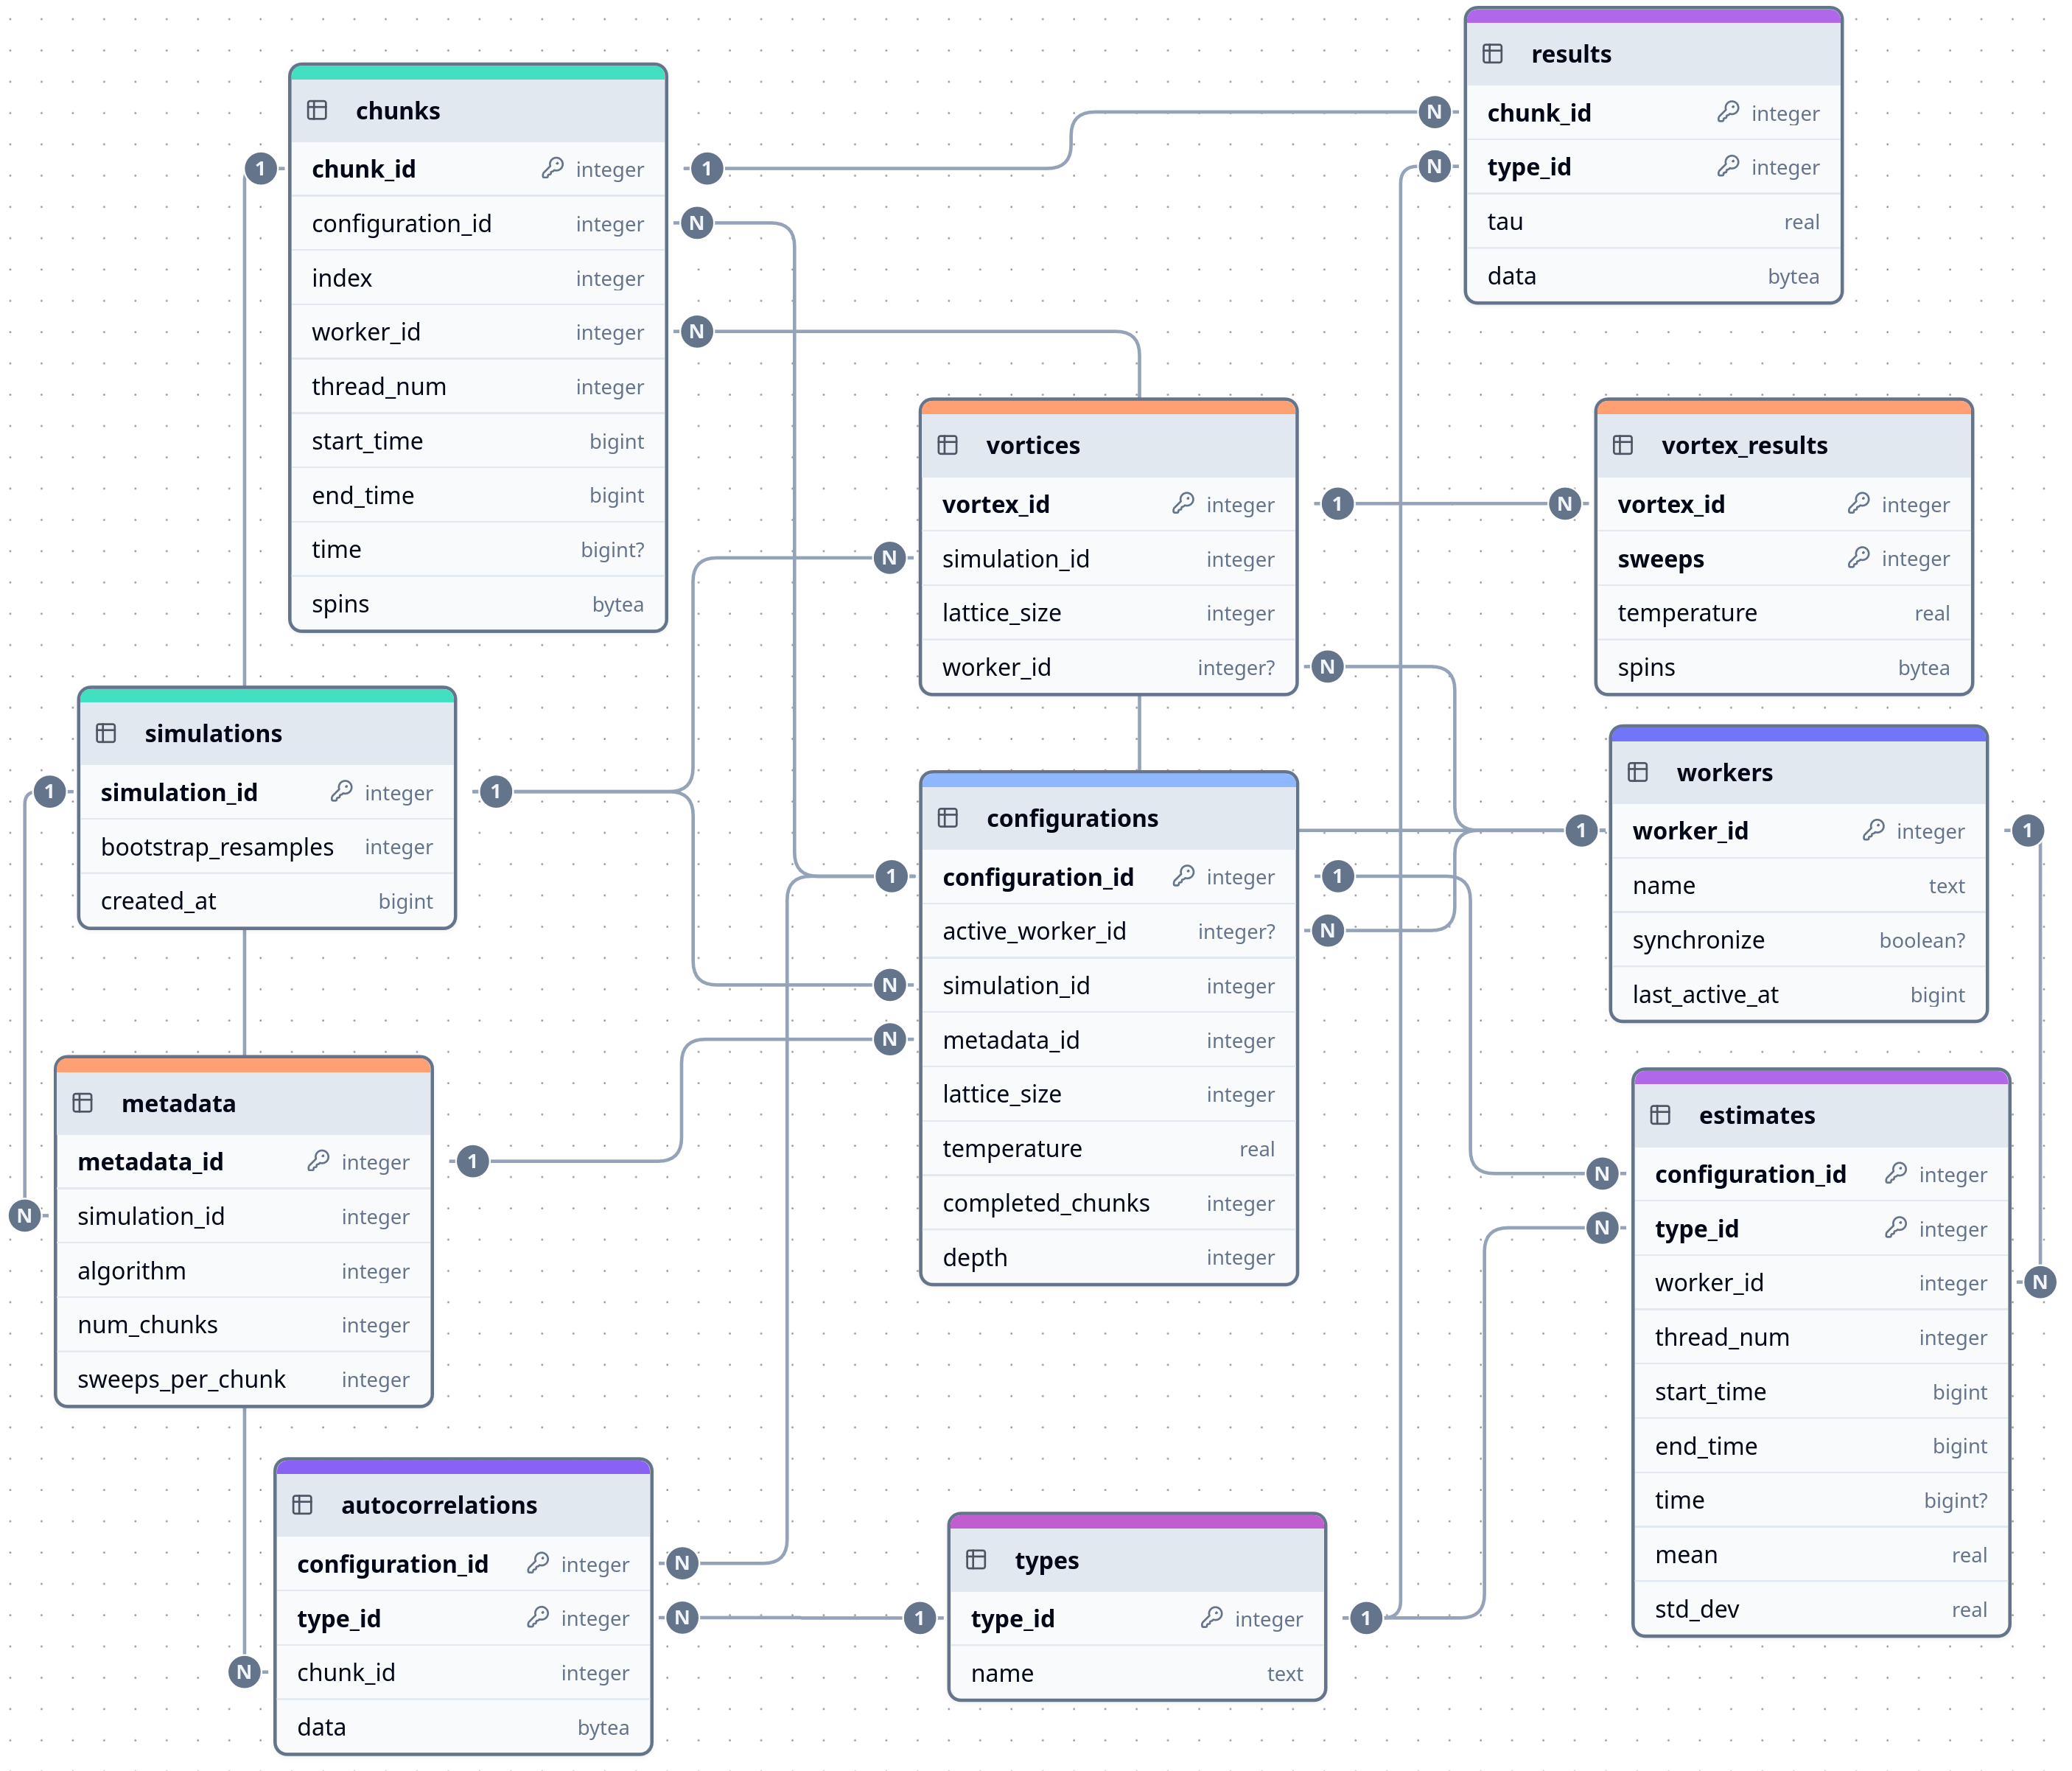
\includegraphics[width=0.8\textwidth]{schema.png}
		\caption[PostgreSQL database schema]{The PostgreSQL database schema for the \emph{data} node.}
		\label{fig:schema}
	\end{figure}
		\chapter{Additional Observables}
	\section{Energy Squared}\label{sec:observables:energy_squared}
		\Observable{Metropolis}{EnergySquare}{energy squared}
		\Observable{Wolff}{EnergySquare}{energy squared}
		
		\Autocorrelation{Metropolis}{EnergySquare}{energy squared}
		\Autocorrelation{Wolff}{EnergySquare}{energy squared}
		
		\IntegratedAutocorrelation{Metropolis}{EnergySquare}{energy squared}
		\IntegratedAutocorrelation{Wolff}{EnergySquare}{energy squared}

	\section{Magnetization Squared}\label{sec:observables:magnetization_squared}
		\Observable{Metropolis}{MagnetizationSquare}{magnetization squared}
		\Observable{Wolff}{MagnetizationSquare}{magnetization squared}
		
		\Autocorrelation{Metropolis}{MagnetizationSquare}{magnetization squared}
		\Autocorrelation{Wolff}{MagnetizationSquare}{magnetization squared}
		
		\IntegratedAutocorrelation{Metropolis}{MagnetizationSquare}{magnetization squared}
		\IntegratedAutocorrelation{Wolff}{MagnetizationSquare}{magnetization squared}

\chapter{Errors}\label{chap:errors}
	\section{Cluster Size}\label{sec:errors:cluster}
		\Error{Metropolis}{Energy}{energy}
		\Error{Wolff}{Energy}{energy}
	
	\section{Energy}\label{sec:errors:energy}
		\Error{Metropolis}{Energy}{energy}
		\Error{Wolff}{Energy}{energy}

	\section{Energy Squared}\label{sec:errors:energysquare}
		\Error{Metropolis}{EnergySquare}{energy squared}
		\Error{Wolff}{EnergySquare}{energy squared}
	
	\section{Specific Heat}\label{sec:errors:specificheat}
		\Error{Metropolis}{SpecificHeat}{specific heat}
		\Error{Wolff}{SpecificHeat}{specific heat}
	
	\section{Helicity Modulus}\label{sec:errors:helicity}
		\Error{Metropolis}{HelicityModulus}{helicity modulus}
		\Error{Wolff}{HelicityModulus}{helicity modulus}
	
	\section{Magnetization}\label{sec:errors:magnetization}
		\Error{Metropolis}{Magnetization}{magnetization}
		\Error{Wolff}{Magnetization}{magnetization}

	\section{Magnetization Squared}\label{sec:errors:magnetizationsquare}
		\Error{Metropolis}{MagnetizationSquare}{magnetization squared}
		\Error{Wolff}{MagnetizationSquare}{magnetization squared}
	
	\section{Magnetic Susceptibility}\label{sec:errors:magneticsusceptibility}
		\Error{Metropolis}{MagneticSusceptibility}{magnetic susceptibility}
		\Error{Wolff}{MagneticSusceptibility}{magnetic susceptibility}
		\chapter{Vortices}\label{chap:vortices}
		\begin{figure}[H]
			\centering
			\begin{subfigure}[h]{0.45\textwidth}
				\centering
				\includegraphics[width=\textwidth]{../figures/Metropolis/frames/1.pdf}
				\caption{At $T=\num{1.5}$, we are in the high-temperature state where the spins are unordered.}
			\end{subfigure}
			~
			\begin{subfigure}[h]{0.45\textwidth}
				\centering
				\includegraphics[width=\textwidth]{../figures/Metropolis/frames/30.pdf}
				\caption{After cooling the system down to $T=\num{0.02}$ there is one bound vortex pair and the rest of the spins are mostly aligned.}
			\end{subfigure}
			\begin{subfigure}[h]{0.45\textwidth}
				\centering
				\includegraphics[width=\textwidth]{../figures/Metropolis/frames/40.pdf}
				\caption{After some sweeps at $T=\num{0.02}$ the vortex pair has come closer together. The rest of the lattice is uniformly aligned.}
			\end{subfigure}
			~
			\begin{subfigure}[h]{0.45\textwidth}
				\centering
				\includegraphics[width=\textwidth]{../figures/Metropolis/frames/59.pdf}
				\caption{After the vortex-antivortex pair has annihilated, a quasi-stable lattice with ordered spins remains.}
			\end{subfigure}
			\caption[Vortex unbinding of vortex-antivortex pairs at low temperatures]{Simulating the process of vortex unbinding by bringing a thermalized high-temperature unordered lattice slowly to low temperatures as described in~\cref{sec:vortex_unbinding}. Below the critical temperature $T_C$ bound vortex-antivortex pairs appear and slowly annihilate at very low temperatures. The lattice is left in a quasi-ordered low-temperature state.}
			\label{fig:vortex_unbinding}
		\end{figure}
		
	\backmatter\pagenumbering{Roman}
		\listoffigures
		\bibliography{refs}
	
\end{document}